\documentclass[../notes.tex]{subfiles}

\pagestyle{main}
\renewcommand{\chaptermark}[1]{\markboth{\chaptername\ \thechapter\ (#1)}{}}
\setcounter{chapter}{3}

\begin{document}




\chapter{Spectroscopy}
\section{IR Selection Rules and Stretching Mode Analysis}
\begin{itemize}
    \item \marginnote{10/17:}Fill out the Google Form to indicate topics we want Wuttig to cover during the review session.
    \item The most common experiments we do to determine normal modes are IR and Raman experiments.
    \begin{itemize}
        \item Vibration modes can be IR and/or Raman active.
        \item IR spectroscopy probes direct absorption of IR light to excite vibrational modes.
        \item We will first determine the IR selection rules.
    \end{itemize}
    \item IR selection rules:
    \begin{itemize}
        \item We want $\Delta v=\pm 1$.
        \item The transition moment integral is for transitions $v\to v'$; it is written as
        \begin{equation*}
            M_{vv'} = \int_{-\infty}^\infty\Psi^*(v')\mu\Psi(v)\dd{x}
        \end{equation*}
        where $\mu$ is the electric dipole moment and $[M_{vv'}]^2$ is the probability of the transition.
    \end{itemize}
    \item If $\mu$ were a constant, then
    \begin{equation*}
        M_{vv'} = \mu\int_{-\infty}^\infty\Psi^*(v')\Psi(v)\dd{x} = 0
    \end{equation*}
    since $\Psi^*(v')$ and $\Psi^*(v)$ are orthogonal functions.
    \begin{itemize}
        \item Therefore, $\mu$ cannot be a constant; it needs to be a function of $x$ and needs to change during the vibration for the transition to be allowed.
    \end{itemize}
    \item A more general form of $[M_{vv'}]^2$ is
    \begin{equation*}
        [M_{vv'}]^2 = \int_\text{all space}\Psi^*(v')\hat{\mu}\Psi(v)\dd\tau
    \end{equation*}
    \begin{itemize}
        \item In order for the above integral to not evaluate to zero, the direct product of the excited state wave function, transition dipole moment, and ground state wave function must contain the totally symmetric IRR. Symbolically,
        \begin{equation*}
            \Gamma_\text{IRR}(\Psi(v'))\times\Gamma_\text{IRR}(\hat{\mu})\times\Gamma_\text{IRR}(\Psi(v))
        \end{equation*}
        decomposes into a sum of IRRs including $A_1$.
    \end{itemize}
    \item Bottom line: A vibration will be IR active if it causes a change in the electric dipole moment of a molecule. A fundamental mode will be IR active if the normal mode which is excited belongs to the same representation as any one or several of the Cartesian coordinates.
    \item What modes are IR active for water?
    \begin{itemize}
        \item Recall that the vibrational modes for \ce{H2O} are $a_1$ corresponding to $\nu_a$, $b_2$ corresponding to $\nu_{as}$, and $a_1$ corresponding to $\delta$.
        \begin{itemize}
            \item Looking at the character table, we notice that both $a_1,b_2$ transform as a linear function ($z,y$, respectively), so all modes are IR active.
            \item More specifically, let's look at $b_2$. If $b_2$ transforms as a linear function, it \emph{is} true that it is IR active. Here's why: If $b_2$ transforms as a linear function, then it will be a component of $\hat{\mu}$. In this case, when we take the direct product $\Gamma_{v'}\times\hat{\mu}$, one term we will evaluate is $b_2\times b_2$. But by the second of the three important theorems, the direct product of any representation times itself will contain the totally symmetric irreducible representation, which is required for IR visibility as per the third of the three important theorems.
        \end{itemize}
        \item Show by direct product analysis that these IR modes are allowed.
        \begin{itemize}
            \item The first transition ($\nu_a$) goes from $a_1\to a_1$ (the ground state is relaxed, hence $a_1$, and the excited state is $\Gamma_\text{vibs}$ for $\nu_a$, which is $a_1$). It follows that
            \begin{equation*}
                \Psi^*(v')\hat{\mu}\Psi(v) \sim\footnote{$\sim$ denotes "transforms as."} a_1
                \begin{pmatrix}
                    a_1\\
                    b_1\\
                    b_2\\
                \end{pmatrix}
                a_1 =
                \begin{pmatrix}
                    a_1\\
                    b_1\\
                    b_2\\
                \end{pmatrix}
            \end{equation*}
            Since the result of our calculation contains the totally symmetric representation (in its first entry), we know that $v_a$ is allowed.
            \item The asymmetric stretch has ground $a_1$ and excited state $b_2$. $\hat{\mu}$ is the same as before.
            \begin{equation*}
                \Psi^*(v')\hat{\mu}\Psi(v) \sim b_2
                \begin{pmatrix}
                    a_1\\
                    b_1\\
                    b_2\\
                \end{pmatrix}
                a_1 =
                \begin{pmatrix}
                    b_2\\
                    a_2\\
                    a_1\\
                \end{pmatrix}
            \end{equation*}
            Since it still contains the all-symmetric wavefunction, it's allowed.
        \end{itemize}
    \end{itemize}
    \item Example:
    \begin{figure}[h!]
        \centering
        \begin{subfigure}[b]{0.2\linewidth}
            \centering
            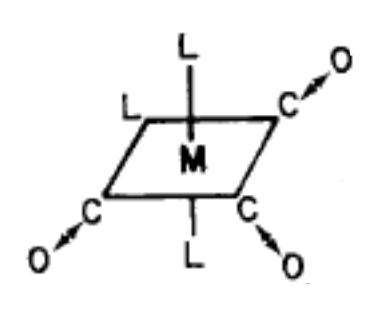
\includegraphics[width=0.8\linewidth]{../ExtFiles/ML3CO3a.png}
            \caption{\emph{mer} isomer.}
            \label{fig:ML3CO3a}
        \end{subfigure}
        \begin{subfigure}[b]{0.2\linewidth}
            \centering
            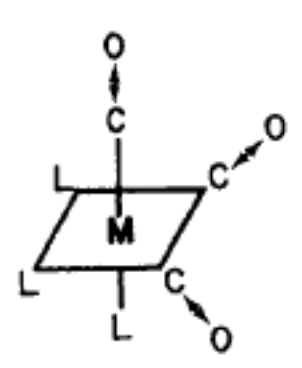
\includegraphics[width=0.8\linewidth]{../ExtFiles/ML3CO3b.png}
            \caption{\emph{fac} isomer.}
            \label{fig:ML3CO3b}
        \end{subfigure}
        \caption{Isomers of an octahedral \ce{ML3(CO)3} complex.}
        \label{fig:ML3CO3}
    \end{figure}
    \begin{enumerate}
        \item Determine the number, symmetries, and IR activities of the carbonyl stretching modes for the two isomers of an octahedral \ce{ML3(CO)3} complex.
        \begin{itemize}
            \item Since we are asked to determine the \emph{carbonyl stretching} modes, we choose as our basis set the three vectors which run parallel to the \ce{CO} bonds in both cases.
            \item The point group of the \emph{mer} isomer is $C_{2v}$; the point group of the \emph{fac} isomer is $C_{3v}$.
            \item With this information, the rest of the question is fairly straightforward.
        \end{itemize}
        \item The IR spectrum of the compound \ce{Mo(CO)3[P(OCH3)3]3} exhibits bands at \qtylist{1993;1919;1890}{\per\centi\meter}. The IR spectrum of compound \ce{Cr(CO)3(CHCH3)3} exhibits bands at \qtylist{1942;1860}{\per\centi\meter}. Based on your answer from part (1), how would you assign the \emph{fac} vs. \emph{mer} structure of these two complexes?
        \begin{itemize}
            \item From part (1), determine which structure gave rise to three nondegenerate stretching modes, and which gave rise to two.
        \end{itemize}
    \end{enumerate}
    \item This example shows that we can determine the stretching modes for just some functional groups.
    \item Be careful with what the basis set is!
    \item Example: Structures for \ce{OsO4N}.
    \begin{itemize}
        \item This molecule has four reasonable structures, having symmetry $C_{2v}$, $C_{3v}$, $C_{4v}$, and $C_s$. It is a great example! Especially when paired with preceding molecules using some subset of these character tables.
    \end{itemize}
\end{itemize}



\section{Raman Selection Rules and Normal Mode Analysis}
\begin{itemize}
    \item \marginnote{10/19:}PSet 2 is due at the beginning of class on Friday.
    \item Raman and IR are complementary, and together they can distinguish geometric possibilities of an unknown molecule.
    \item \textbf{Raman spectroscopy}: A type of spectroscopy which probes inelastic scattering of light where the loss in energy corresponds to a vibrational frequency (\textbf{Stokes shift}).
    \item In Raman, you go to \textbf{virtual energy states}.
    \item \textbf{Virtual energy state}: The coupling of a photon with a high energy state.
    \item \textbf{Rayleigh scattering}: The amount of energy put in is the amount of energy you get out. \emph{Also known as} \textbf{elastic scattering}.
    \begin{itemize}
        \item Doesn't give us a change, so we filter this out.
    \end{itemize}
    \item \textbf{Stokes Raman scattering}: The photon out has less energy than the photon in; some energy was scattered.
    \begin{itemize}
        \item We excite from the ground state to a virtual energy state, and then fall back down but not all the way to the ground state, i.e., the electron remains in an excited state even after emitting its photon.
    \end{itemize}
    \item \textbf{Anti-Stokes Raman scattering}: The photon out has more energy than the photon in; we start at a higher energy state and then fall back to ground.
    \begin{itemize}
        \item We excite from an excited state to a virtual energy state, and the fall back down all the way to the ground state.
    \end{itemize}
    \item A vibrational mode will be Raman active if the polarizability of the molecule changes during the vibration. A fundamental transition will be Raman active (i.e., will give rise to a Raman shift) if the normal mode involved belongs to the same representation as one or more of the components of the polarizability tensor of the molecule.
    \item Transition probability in Raman:
    \begin{equation*}
        M_w^2 = \left[ \int_{-\infty}^\infty\Psi_{v'}^*\hat{\alpha}\Phi_v\dd\tau \right]^2
    \end{equation*}
    \begin{itemize}
        \item Polarizability describes the shape of the electron cloud and can be described by a tensor.
        \begin{equation*}
            \begin{bmatrix}
                \mu_x\\
                \mu_y\\
                \mu_z\\
            \end{bmatrix}
            =
            \begin{bmatrix}
                \alpha_{xx} & \alpha_{xy} & \alpha_{xz}\\
                \alpha_{yx} & \alpha_{yy} & \alpha_{yz}\\
                \alpha_{zx} & \alpha_{zy} & \alpha_{zz}\\
            \end{bmatrix}
            \begin{bmatrix}
                E_x\\
                E_y\\
                E_z\\
            \end{bmatrix}
        \end{equation*}
        \item The matrix above is the polarizability tensor, and the right vector above describes the electric field.
        \item Three $\alpha$ values are redundant: The matrix above is symmetric, so
        \begin{align*}
            \alpha_{xz} &= \alpha_{zx}&
            \alpha_{yz} &= \alpha_{zy}&
            \alpha_{yx} &= \alpha_{xy}
        \end{align*}
        \item Thus, $\hat{\alpha}$ has six different components.
        \item If you do the math, you learn that the transition is allowed if the symmetric IRR is in the direct product and the normal mode is a quadratic function.
    \end{itemize}
    \item Recall: Linear for IR, quadratic for Raman.
    \item Example: The nine modes of vibration, two pairs of which are degenerate, are derived below for \ce{XeF4}. Show that the $b_{1g}$ fundamental transition is allowed for Raman but forbidden for infrared.
    \begin{equation*}
        \Gamma_\text{vibs} = a_{1g}+b_{1g}+b_{2g}+a_{2g}+a_{2u}+b_{2u}+2e_u
    \end{equation*}
    \begin{itemize}
        \item Checking the $D_{4h}$ character table, we see that the two linear representations are $a_{2u}$ and $e_u$. Thus,
        \begin{equation*}
            \Psi^*_{v'}\hat{\mu}\Psi_v \sim b_{1g}
            \begin{pmatrix}
                a_{2u}\\
                e_u\\
            \end{pmatrix}
            a_{1g} =
            \begin{pmatrix}
                b_{2u}\\
                e_u\\
            \end{pmatrix}
        \end{equation*}
        Thus, since $a_{1g}$ doesn't appear, the IR transition is not allowed.
        \item Checking the $D_{4h}$ character table, we see that the four quadratic representations are $a_{1g}$, $b_{1g}$, $b_{2g}$, and $e_g$. Thus,
        \begin{equation*}
            \Psi^*_{v'}\hat{\mu}\Psi_v \sim b_{1g}
            \begin{pmatrix}
                a_{1g}\\
                b_{1g}\\
                b_{2g}\\
                e_g\\
            \end{pmatrix}
            a_{1g} =
            \begin{pmatrix}
                b_{1g}\\
                a_{1g}\\
                a_{2g}\\
                e_g\\
            \end{pmatrix}
        \end{equation*}
        Thus, since $a_{1g}$ appears, the Raman transition is allowed.
    \end{itemize}
    \item \textbf{Fundamental transition}: A transition starting from the ground state.
    \begin{itemize}
        \item $\Psi_v$ is always the totally symmetric IRR for a fundamental transition.
        \item The wording "$b_{1g}$ fundamental transition" in the previous example means "the transition form $a_{1g}$ to $b_{1g}$."
        \item Essentially, we're not dealing with overtones, not starting from an excited state, no coupling, nothing fancy.
        \item We will briefly talk about overtones later.
    \end{itemize}
    \item Example: Determine the symmetries and activities of the normal modes of vibration for the cyclopropenyl cation. Use all atoms ($N=6$), i.e., use the Cartesion displacement method.
    \begin{itemize}
        \item Point group: $D_{3h}$.
        \item $\Gamma_{xyz}=(3,0,-1,1,-2,1)$.
        \item $\Gamma_\text{unmoved}=(6,0,2,6,0,2)$.
        \item $\Gamma_{3N}=(18,0,-2,6,0,2)=2A_1'+2A_2'+4E'+2A_2'+2E'$.
        \item $\Gamma_\text{vibs}=2A_1'+A_2'+3E'+A_2''+E''$.
        \item Operators:
        \begin{align*}
            \hat{\mu} &=
            \begin{pmatrix}
                e'\\
                a_2''\\
            \end{pmatrix}&
            \hat{\alpha} &=
            \begin{pmatrix}
                a_1'\\
                e'\\
                e''\\
            \end{pmatrix}
        \end{align*}
        \item $a_1'$ is Raman active, $e'$ is both, $a_2''$ is IR active, and $e''$ is both.
    \end{itemize}
    \item You only need uppercase Mulliken symbols for character tables and Tanabe-Sugano diagrams.
    \item \textbf{Rule of mutual exclusion}: No normal modes can be both infrared and Raman active in a molecule that possesses a center of symmetry.
    \item Question: Spectrum analysis. What symmetry element must be present?
    \begin{itemize}
        \item Observation: Lack of coincidental IR and Raman peaks in the spectra of benzene.
        \item Thus, no linear bases or quadratic bases overlap. The linear must all be $-1$ and the quadratic must all be 1.
        \item Thus, an inversion $i$ is present.
    \end{itemize}
\end{itemize}




\end{document}